\documentclass[9pt,twocolumn,twoside]{../../styles/osajnl}
\usepackage{fancyvrb}
\journal{i524} 

\title{ On-line advertisement click prediction - Project proposal }

\author[1,*]{Sahiti Korrapati}

\affil[1]{School of Informatics and Computing, Bloomington, IN 47408, U.S.A.}

\affil[*]{Corresponding authors: sakorrap@iu.edu, S17-IR-2013}

\dates{S17-IR-2013, May 04, 2017}

\ociscodes{Hadoop, Ad click Prediction, BigData, Ansible, Chameleon cloud, Apache Pig, HDFS, MapReduce}

% replace this with your url in github/gitlab
\doi{\url{https://github.com/laszewsk/sp17-i524/blob/master/project/S17-IR-2013/report/report.pdf}}

\begin{abstract}
This project aims at predicting the most suitable advertisements to be displayed on the web pages. Advertisements are selected based on the relevance. Relevance factor is calculated by ranking each ad based on the likelihood of clicking the ad if displayed. Data is obtained as CSV files from Kaggle Data sets and is stored in Hadoop Data File system(HDFS). In this project, Ansible along with Cloud mesh is used to deploy cloud architecture and the necessary soft wares on Chameleon cloud. For data exploration and analysis, as the dataset is huge in the order of 100s of gigabytes Apache Pig on Hadoop is chosen. The Pig engine in can execute the data flows in parallel by making use of Hadoop MapReduce framework.
\newline
\end{abstract}
\setboolean{displaycopyright}{true}

\begin{document}

\maketitle

\section{Introduction}
It has been analyzed that an average American spends about 23 hours per week surfing on-line \cite{news-social-media}. This on-line user activity is being captured by companies to perform analyzes for advertisement, recommendations and many other purposes. This has given rise to the field of "Web Analytics" and one such application is Ad Click prediction.

Many measures are available to asses the ad performance. One popular measure to asses the immediate ad response is click-through rate (CTR) of the advertisement \cite{dictionary-clickThrough} which is defined as the ratio of number of clicks on an ad to the number of times the ad is shown, expressed as a percentage. In this project, I attempted to make use of CTR along with ranking each ad based on the level of relevance to the original web page. For calculating the CTR, historical data of user activity needed to be explored. \cite{wiki-clickThrough}.

The user activity data from web that is used for prediction is enormous. Every page view, advertisement and click is being tracked by web browsers, and that level of data for millions of users potentially generates enormous volumes. The current internet giants use big data technologies to handle such large volumes of data. The current project uses Apache pig along with Hadoop for analyzing and for prediction. Hadoop is a large scale data processing system which runs on parallal processing to handle huge volumes of data. Pig is a high level language which runs on top of Hadoop's HDFS infrastructure. Pig Latin scripts are simple to comprehend and SQL-like queries which can process large volumes of data.

Ansible along with Cloudmesh is used to deploy the software and chameleon cloud for running virtual machines. Ansible is a cloud automation tool which allows easy deployment and configuration of multiple servers in one step. Cloudmesh allows us to deploy and install Hadoop instances on a cluster with any number of nodes.

\section{Background}
\subsection{About Data}
The data set in this paper is taken from kaggle datasets. It is released by Outbrain which has 2 Billion page views and 16,900,000 clicks of 700 Million unique users, across 560 sites \cite{kaggle-outbrain}.

The dataset contains a sample of users’ page views and clicks, as observed on multiple publisher sites in the United States between 14-June-2016 and 28-June-2016. Each viewed page or clicked recommendation is further accompanied by some semantic attributes of those documents \cite{kaggle-outbrain}. It contains numerous sets of content recommendations served to a specific user in a specific context. Each context (i.e. a set of recommendations) is given a display\_id. In each such set, the user has clicked on at least one recommendation. Our task is to rank the recommendations in each group by decreasing predicted likelihood of being clicked \cite{kaggle-outbrain}.

Each user in the dataset is represented by a unique id (uuid). A person can view a document (document\_id), which is simply a web page with content (e.g.  a news article). On each document, a set of ads (ad\_id) are displayed. Each ad belongs to a campaign (campaign\_id) run by an advertiser (advertiser\_id). Figure \ref{fig:OutbrainData} shows the fields in our dataset. Metadata about the document is also provided, such as which entities are mentioned, a taxonomy of categories, the topics mentioned, and the publisher \cite{kaggle-outbrain}.

\begin{figure}[hptb]
\centering
\includegraphics[width=\linewidth]{images/page_view.png}
\caption{Displaying Source, Publisher, Document, Promoted content set and items \cite{kaggle-outbrain}}
\label{fig:OutbrainData}
\end{figure}

\subsection{Ansible and Cloudmesh client toolkit}
Ansible is an opensource cluster management tool which has the ability to maintain a fully immutable server architecture and design. It is a simple automation engine that automates cloud provisioning, configuration management, application deployment, intra-service orchestration \cite{www-ansible-work}. It doesn't use agents or custom security infrastructure, so it's easy to deploy by using "YAML-language" (YAML, in the form of Ansible Playbooks). 

Using Ansible, users can define any number of IP Addresses in hosts file, and create custom groups for specific tasks. These group names can be referred in the YAML file to perform specific set of tasks in each of the virtual machines. Ansible also has options to define specific roles for each task and make YAML files dynamic using global variables.

With Cloud mesh, the deployment becomes even simpler and easier. Cloud mesh client toolkit, a lightweight client interface to access heterogeneous clouds, clusters, and workstations, available as API, commandline client and commandline shell. Their quick start user manual has everything that is needed to start using the tool \cite{www-cm-docs}.

The current project uses Cloudmesh's "cm" command to perform multiple tasks including deployment of cluster, installing and configuring Hadoop and Pig, enabling the cloud nodes to be able to ssh with each other and assigning floating IP addresses to each node. The configuration of the cluster can be defined in Cloudmesh's YAML file and accordingly the cluster will be created with the given OS and type.

\subsection{Hadoop in Big-data}
Hadoop is a distributed platform designed to help manage and analyze massive data-sets that are too big or costly to put in relational databases. Rather than storing and processing the whole data in one high-end computer, data can be spread across many smaller nodes. By spreading the data across multiple nodes, the storage as well computational speed can be scaled by parallel processing \cite{www-thinkbig}.

Hadoop framework is developed for distributed processing of large data sets across clusters of computers using simple programming models. It can scale up from single servers to thousands of machines, each offering local computation and storage. The library is designed to deliver a highly available service on top of a cluster of computers, each of which may be prone to failures \cite{www-readwrite}.

\subsection{HDFS and MapReduce}
Hadoop Distributed File System (HDFS) and the MapReduce parallel processing framework are two primary components at the core of Apache Hadoop. Figure \ref{fig:HadoopArchitecture} shows the high level architecture of Hadoop in regards to HDFS and MapReduce 

\begin{figure}[hptb]
\centering
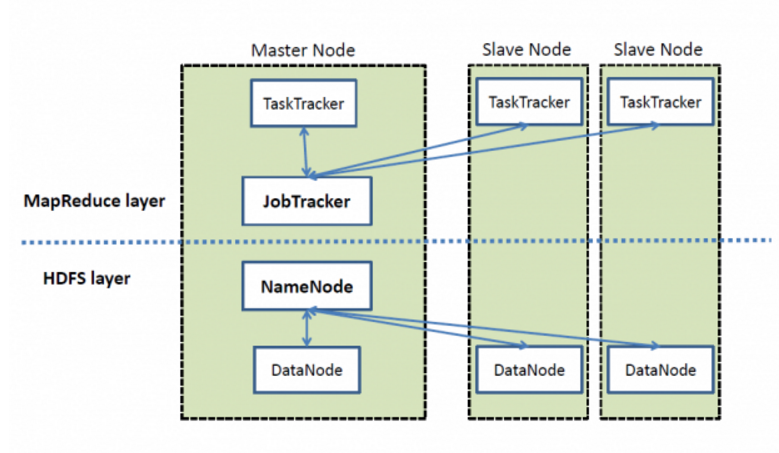
\includegraphics[width=\linewidth]{images/HadoopArch.PNG}
\caption{ High Level Architecture of Hadoop \cite{www-opensource}}
\label{fig:HadoopArchitecture}
\end{figure}

HDFS is a distributed, scalable, and portable file-system for Hadoop framework.
Files are broken into blocks and spread across nodes in the cluster in HDFS. The blocks are also replicated on different nodes so that even if one of the nodes fails another one of the live nodes still has a copy of the data. There is a NameNode and DataNodes. The NameNode maintains the references on the file split up in blocks across nodes in the cluster. While reading, client process contacts the NameNode for this metadata and ask the corresponding DataNodes for those blocks for reading \cite{www-thinkbig}.
MapReduce is for processing files stored in a distributed environment like HDFS. A typical MapReduce application has two functions, a Mapper and a Reducer. Mappers and Reducers run as tasks on nodes in the cluster. Two processes JobTracker and TaskTracker manages MapReduce framework. The JobTracker is the master process that coordinates the Map and Reduce tasks sent across the cluster.

\subsection{Apache Pig}
Pig platform is designed to work with large data sets for analysis. The Pig dialect is called Pig Latin, and the Pig Latin commands get compiled into MapReduce jobs that can be run on a suitable platform, like Hadoop. Figure \ref{fig:Pig} illustrates how it makes use of MapReduce framework.

\begin{figure}[hptb]
\centering
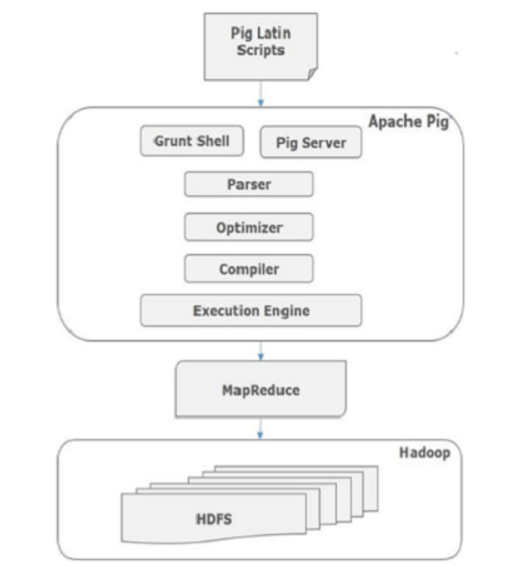
\includegraphics[width=\linewidth]{images/PigArch.PNG}
\caption{ Architecture of Apache Pig \cite{www-opensource}}
\label{fig:Pig}
\end{figure}

Pig is a high level language which is similar to SQL in syntax. The structure of Pig is designed such that the Pig scripts are made amenable for parallel processing. Pig scripts are automatically optimized so that the programmers can focus on semantics rather than efficiency \cite{www-pig-apache}. Pig also has options to create user defined functions to perform complex tasks using Pig.

\subsection{Chameleon cloud}
Chameleon Cloud is a cloud platform offered for research purposes free of charge. It is maintained by the Chameleon community, and is funded exclusively for use by students and faculty by the National Science Foundation. Chameleon Cloud is deployed at University of Chicago and Texas Advanced Computing Center, and consists 650 multi-core cloud nodes, 5PB of total disk space, and leverage 100 Gbps connection between the sites. 

The current project uses a cluster created on Chameleon cloud instance with three virtual machines on which Hadoop operates. Ubuntu 14.04 was installed on these machines with 20 GB disk space and 2 GB ram each.

\subsection{Data Analysis}
Even though we have page\_views data, I have excluded that from analysis. As the data was in orders of 100s of gigabytes for just 2 weeks. With the resources available, I can only take two days of data for analysis. The prediction will be of very low confidence if only two days are considered. Since, I wanted to produce a useful prediction of Ad ids, I chose to predict the more linkely adS by relevance factor. For which data was analyzed using Apache Pig in the MapReduce mode. The datasets clicks\_train and events were joined to get a list of documents to make the predictions. The above list was joined to documents\_events, documents\_categories and documents\_topics to generate a master dataset of all the required documents, their topics, categories and entities. The dataset promoted\_content was joined with documents\_events, documents\_categories and documents\_topics to generate a dataset which has all advertisement ids, and their related document entitiy, topic and category. A master join between the two datasets on the event, topic and category ID was performed to get matching document IDs. On this data, relevancy score for each match, by multiplying the confidence levels. The final dataset is grouped by document ID and select top 6 matching ads based on relevancy score. The top 6 ads are the recommendations to be shown on each page. This recommendation engine is purely based on the matching document properties.

\section{Setup and Configuration}
This project was setup using Ansible and Cloudmesh Client. Cloudmesh client was used to install and deploy Hadoop clusters on Chameleon Cloud. Ansible was then configured to perform a set of tasks on the namenode of the server. File movement was handled using Ansible playbooks. The final Pig script was run on the namenode Hadoop server using automated Ansible scripts.

The configuration for the cluster deployed is given in Table 1. The project uses three virtual machines defined on Chameleon Cloud. One of them acted as namenode while the rest acted as datanodes. 

\begin{table}
\begin{tabular}{|c|c|}
\hline
    Server & Ubuntu14.04 \\ \hline
    VCPU & 2 \\\hline
    Ram & 4 GB \\\hline
    Disk & 40 GB\\\hline
\end{tabular}
\caption{Virtual Machine Configuration}
\end{table}
\section{Work Flow}

The deployment of clusters was done using Cloudmesh client's "cm deploy" command. This automatically created a three node Hadoop cluster and enabled cross SSH between the nodes so that they will be able to communicate with each other. Next step was to use Ansible to transfer the data files and Pig script to cloud. Once this data transfer was done, Ansible scripts were used to move the files from cloud to hdfs dfs repository. The pig script was run using Ansible from local system and timed for benchmarking. The final step was to transfer the files back from hdfs to local system using Ansible.

\section{Experiments and Results}
Multiple experiments were conducted using different sizes of input data and the time results were used to benchmark Chameleon Client for this particular analysis. The data size was taken for predicting the most likely to be clicked for 100, 2000, 5000, 10000 webpages. Each document ID corresponds to a page that needs predictions and a list 6 Ad\_id are predicted for each document\_id based on relevance factor calculated.
The results are presented in  \ref{fig:regular}.  

The graphs are plotted for time versus number of webpages to which predictions are made (\# documents). It is evident from \ref{fig:regular}, the time required to predict is linearly proportional to number of webpages. This shows that the time complexity is O(n) where n is number of document ids.


\begin{figure}[hptb]
\centering
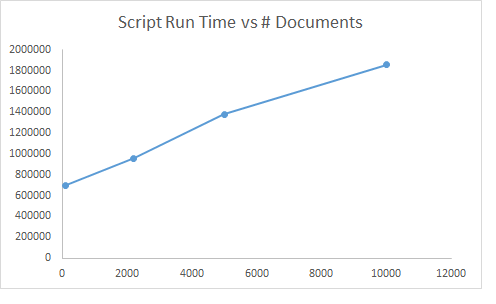
\includegraphics[width=\linewidth]{images/regular.png}
\caption{ Benchmarking Results: Time(in Milliseconds) taken for predicting Best 6 Ads for webpages}
\label{fig:regular}
\end{figure}

\section{Conclusion}
Apache Hadoop technologies can be used to process large volumes of data parallely to make quick analyses. Apache Pig is an addon for Hadoop, which is a high level language for writing queries to process data. Apache Pig is efficient in query optimization and enables parallelism for its processing. The current project uses Apache Hadoop and Pig to process large datasets related to online ad prediction. Online advertisement is one space where large amounts of data is collected and it demands the use of Hadoop like parallel processing systems to get meaningful insights from the data. 

As we can see from the results, Apache Pig was able to handle reasonably large sized files in short times. The processing time increases as the input query size increases. This is a small cluster of three nodes and it is able to process such large volumes of data efficiently. These nodes can be horizontally expanded to utilize the full extent of Hadoop's parallel processing capabilities in order to scale up. 

\section{Future work}
Planning to conduct predictions based on Ensemble methods. One way to predict is through click-through rate and one way is to predict by relevance factor. Using relevance factor as one of the attributes alng with platform, user id and geo-location, logistic regression can be run to predict if the top ad ids generated by relevance factor to be included in the list or not. Since, all that information is given in page\_views file which is in order of 100s of gigabytes for just 2 weeks data, we need large clusters. 

\section*{Acknowledgements}

The authors thank Professor Gregor Von Laszewski and all the AIs of big data class for the guidance and technical support.

% Bibliography
\bibliography{references}
 
\section*{Author Biographies}
\begingroup
\setlength\intextsep{0pt}
\begin{minipage}[t][3.2cm][t]{1.0\columnwidth} % Adjust height [3.2cm] as required for separation of bio photos.
  \noindent
  {\bfseries Sahiti Korrapati} is pursuing her MSc in Data Science from
  Indiana University Bloomington
\end{minipage}
\endgroup
\end{document}

